\documentclass[12pt]{article}


\usepackage{amssymb}
\usepackage{amsmath}
\usepackage{fullpage}
\usepackage{epsfig}
\usepackage{epstopdf}
\everymath{\displaystyle}
\usepackage{enumerate}



\begin{document}

\begin{center}
\underline{\Large{Chapters 2.1-2.3: Pythagorean Theorem, Distance Formula, \& Circles}}
\end{center}

\subsection*{Expected Skills:}

\begin{itemize}

\item Given the lengths of two sides of a right triangle, be able to use the Pythagorean Theorem to determine the length of the remaining side.

\item Be able to calculate the distance between two points in the plane.

\item Be able to write an equation of a circle which satisfies some given conditions.  Also, be able to identify the center and radius of a circle.

\item Be able to find the point on a curve which is closest to or farthest from a given point $P$.

\end{itemize}

\subsection*{Practice Problems: }

\begin{enumerate}

\item For the triangle below, determine the lengths of the two unlabeled sides.
\begin{center}
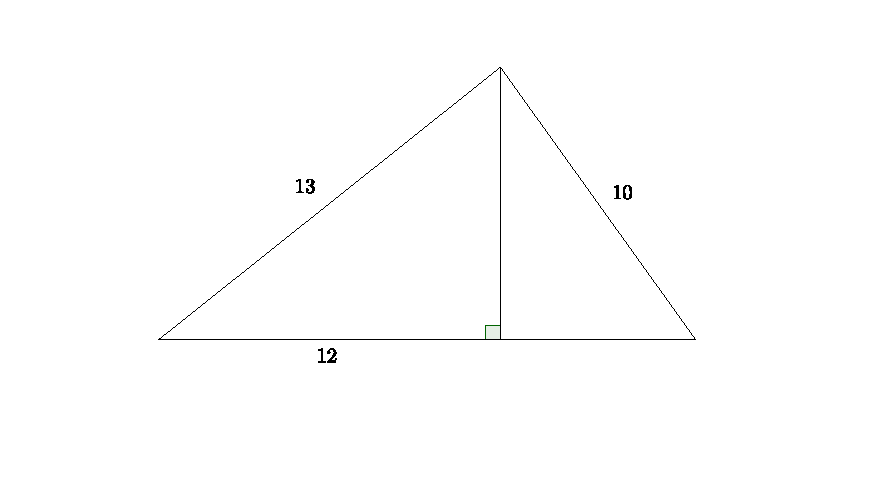
\includegraphics[scale=.8]{triangle1.pdf}
\end{center}

\includegraphics[scale=0.5]{start.pdf}
{{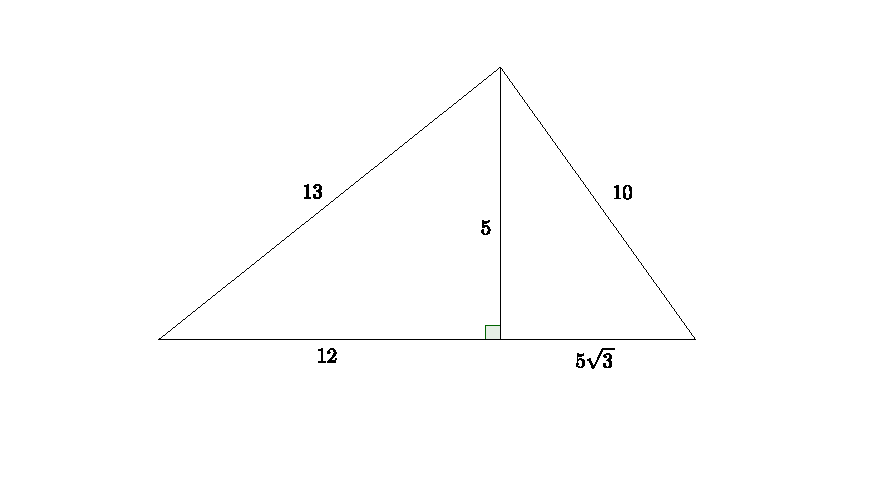
\includegraphics[scale=0.6]{triangle2.pdf}}}
\includegraphics[scale=0.5]{end.pdf}


\item Televisions are advertised by the length of the screen's diagonal.  A television has a rectangular screen with a height of 36 inches and a length of 64 inches.  How should this television be advertised?

\includegraphics[scale=0.5]{start.pdf}
{{$4\sqrt{337}\approx73.43$ inches}}
\includegraphics[scale=0.5]{end.pdf}


\item A ladder of length 25 feet is leaning against a vertical wall.  The ladder is initially 7 feet from the wall; but, it is being pushed towards the wall at a constant rate of 2 feet per second.  This causes the top of the ladder to slide up the wall. 
\begin{enumerate}
\item How high above the ground is the top of the ladder initially?

\includegraphics[scale=0.5]{start.pdf}
{24 feet}
\includegraphics[scale=0.5]{end.pdf}


\item How high above the ground is the top of the ladder after 1 second has elapsed?

\includegraphics[scale=0.5]{start.pdf}
{$10\sqrt{6}$ feet}
\includegraphics[scale=0.5]{end.pdf}


\end{enumerate}

\item Let $T$ be the triangle with vertices $A(0,0)$, $B(8,0)$, and $C(4,4\sqrt{3})$.

\begin{enumerate}

\item Show that $T$ is an equilateral triangle.

\includegraphics[scale=0.5]{start.pdf}
{{1\linewidth}{We will calculate the lengths of all three sides and verify that they are equal.
\begin{itemize}
\item $d_{AB}=8$
\item $d_{AC}=\sqrt{(4-0)^2+(4\sqrt{3}-0)^2}=8$
\item $d_{BC}=\sqrt{(4-8)^2+(4\sqrt{3}-0)^2}=8$
\end{itemize}}}
\includegraphics[scale=0.5]{end.pdf}


\item Show that the area of an equilateral triangle with sides of length $s$ is $A=\frac{\sqrt{3}}{4}s^2$.

\includegraphics[scale=0.5]{start.pdf}
{{1\linewidth}{Recall that the area of a triangle is $A=\frac{1}{2}bh$ and consider the triangle shown below.
\begin{center}
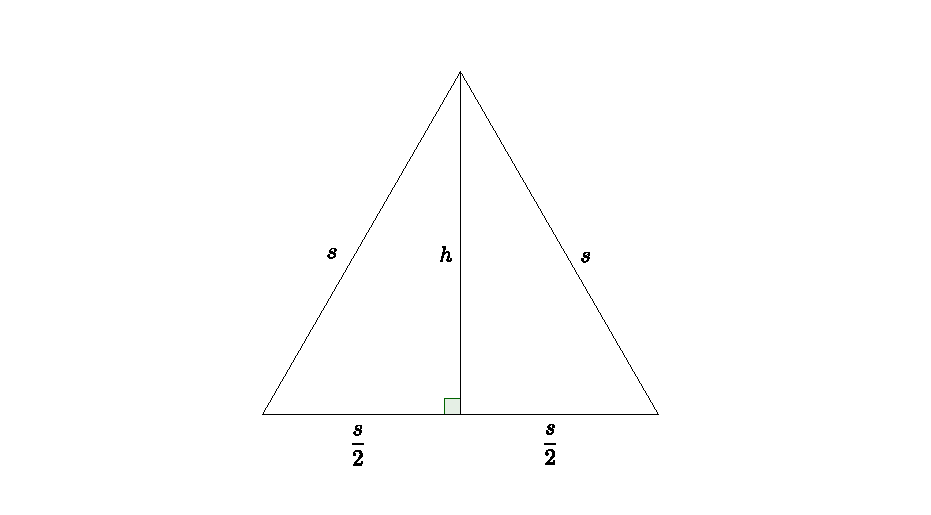
\includegraphics[scale=0.5]{equilateral.pdf}
\end{center}
The length of the base is $s$.  Using the Pythagorean Theorem, you can determine that the height is $h=\frac{\sqrt{3}}{2}s$.  Thus, the area is $A=\frac{1}{2}(s)\left(\frac{\sqrt{3}}{2}s\right)=\frac{\sqrt{3}}{4}s^2$.}}
\includegraphics[scale=0.5]{end.pdf}


\item What is the area of $T$?

\includegraphics[scale=0.5]{start.pdf}
{$16\sqrt{3}$}
\includegraphics[scale=0.5]{end.pdf}


\end{enumerate}

\newpage

\item What is the area of a square inscribed in a unit circle?

\includegraphics[scale=0.5]{start.pdf}
{{1\linewidth}{The area is 2. Hint: consider the following diagram.
\begin{center}
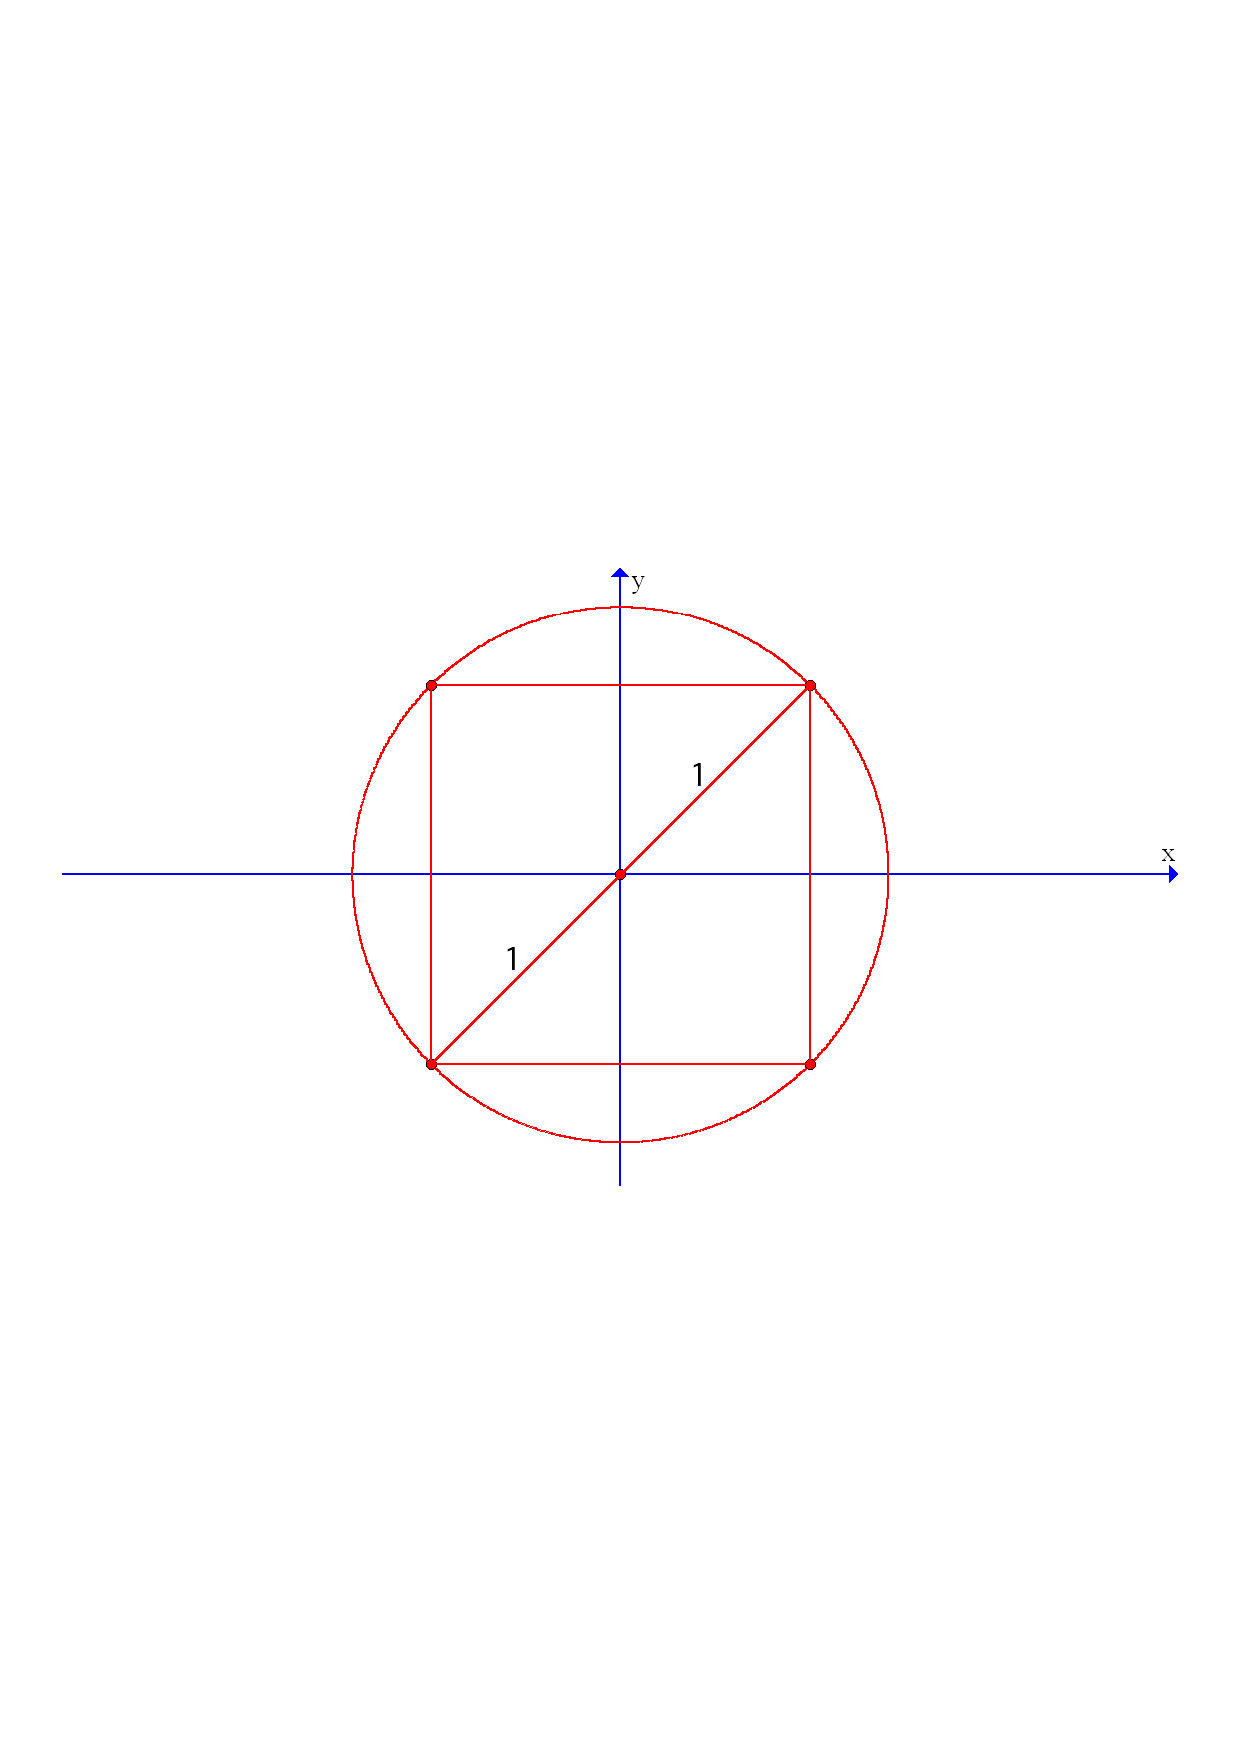
\includegraphics[scale=0.5]{inscribed.pdf}
\end{center}}}
\includegraphics[scale=0.5]{end.pdf}


\item Find an equation of the circle which has a center of $(3,5)$ and which has a radius of 6.

\includegraphics[scale=0.5]{start.pdf}
{$(x-3)^2+(y-5)^2=36$}
\includegraphics[scale=0.5]{end.pdf}


\item Suppose $A(1,5)$ and $B(3,-2)$ are endpoints of a diameter of a circle.  Find an equation of this circle.

\includegraphics[scale=0.5]{start.pdf}
{$(x-2)^2+\left(y-\frac{3}{2}\right)^2=\frac{53}{4}$}
\includegraphics[scale=0.5]{end.pdf}


\item The set of points in the $xy$-plane which satisfy $x^2-2x+y^2+10y=-17$ forms a circle.

\begin{enumerate}

\item What are the center and radius of this circle?

\includegraphics[scale=0.5]{start.pdf}
{Center $(1,-5)$, radius $r=3$}
\includegraphics[scale=0.5]{end.pdf}


\item Does the origin lie inside or outside this circle?  Explain.

\includegraphics[scale=0.5]{start.pdf}
{{The origin is outside of the circle.}}
\includegraphics[scale=0.5]{end.pdf}


\end{enumerate}

\item Consider the square which is centered at the origin and has sides of length $2$ which are parallel to the coordinate axes.

\begin{enumerate}

\item Find an equation of the circle which is inscribed within this square.

\includegraphics[scale=0.5]{start.pdf}
{{$x^2+y^2=1$}}
\includegraphics[scale=0.5]{end.pdf}


\item Find an equation of the circle which is circumscribed around this square.

\includegraphics[scale=0.5]{start.pdf}
{{$x^2+y^2=2$}}
\includegraphics[scale=0.5]{end.pdf}


\end{enumerate}

\item Find equations of the two tangent circles of equal radii which have centers $C_1(-2,5)$ and $C_2(3,4)$, respectively.

\includegraphics[scale=0.5]{start.pdf}
{{$(x+2)^2+(y-5)^2=\frac{13}{2}$ and $(x-3)^2+(y-4)^2=\frac{13}{2}$}}
\includegraphics[scale=0.5]{end.pdf}


\item Consider the circle of radius $r$ shown below:

\begin{center}
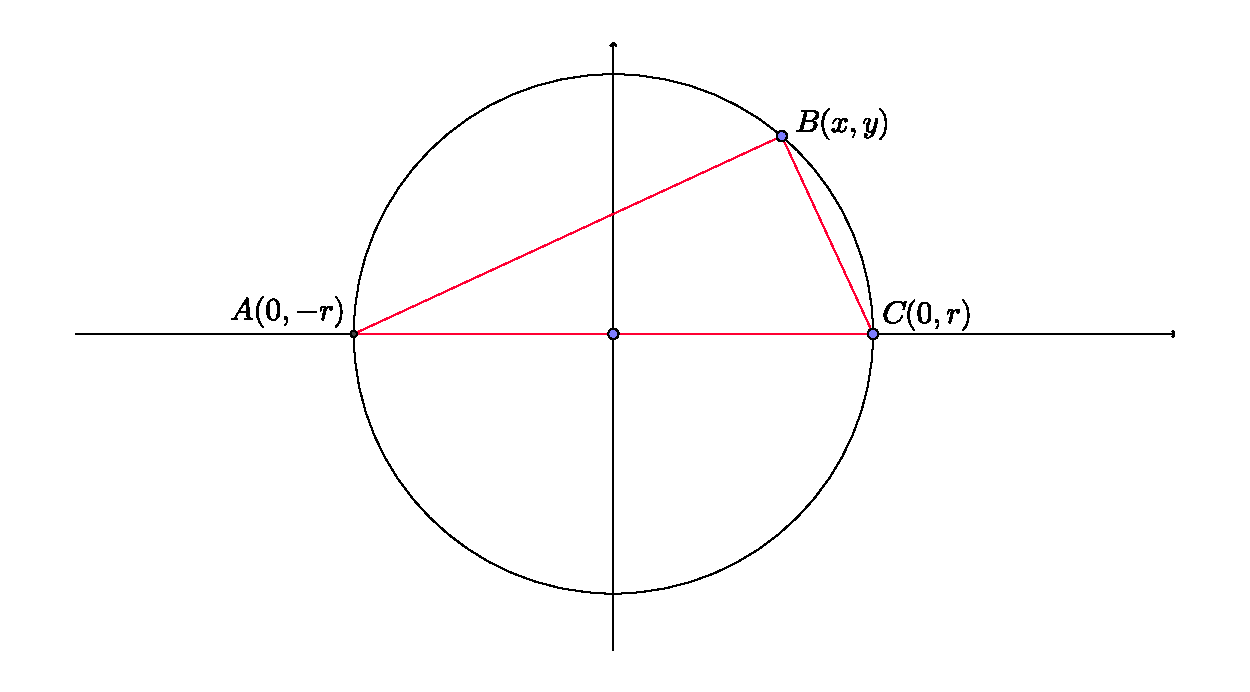
\includegraphics[scale=0.5]{circle.pdf}
\end{center}

\begin{enumerate}

\item Calculate $d_{AB}$, $d_{BC}$, and $d_{AC}$.  

\includegraphics[scale=0.5]{start.pdf}
{{{1\linewidth}{Using the distance formula, we calculate the required lengths:
\begin{itemize}
\item $d_{AB}=\sqrt{(x-0)^2+(y+r)^2}=\sqrt{x^2+(y+r)^2}$
\item $d_{BC}=\sqrt{(0-x)^2+(r-y)^2}=\sqrt{x^2+(r-y)^2}$
\item $d_{AC}=2r$
\end{itemize}}}}
\includegraphics[scale=0.5]{end.pdf}


\item Use your result from part (a) to argue that $\triangle ABC$ is a right triangle.  (This is Thales' Theorem.)

\includegraphics[scale=0.5]{start.pdf}
{{{1\linewidth}{We will show that $(d_{BC})^2+(d_{AB})^2=(d_{AC})^2$.  At some point in our calculation, we will use the fact that the circle has equation $x^2+y^2=r^2$.
\begin{align*}
(d_{BC})^2+(d_{AB})^2 &=\left(\sqrt{x^2+(r-y)^2}\right)^2+\left(\sqrt{x^2+(y+r)^2}\right)^2\\
&=x^2+(r-y)^2+x^2+(y+r)^2\\
&=x^2+r^2-2ry+y^2++x^2 +y^2+2ry+r^2\\
&=2(x^2+y^2)+2r^2\\
&=2r^2+2r^2 \\
&=4r^2\\
&=(d_{AC})^2
\end{align*}
Thus, since the Pythagorean Theorem is satisfied, $\triangle ABC$ is a right triangle.
}}}
\includegraphics[scale=0.5]{end.pdf}


\end{enumerate}

\item Consider the curve $y=\sqrt{x}$ on $[0,10]$ and the point $P(9.5,0)$

\begin{enumerate}

\item Find the point on the curve which is closest to $P$.

\includegraphics[scale=0.5]{start.pdf}
{{$(9,3)$ which is a distance of $\frac{1}{2}\sqrt{37}$ from $P$.}}
\includegraphics[scale=0.5]{end.pdf}


\item Find the point on the curve which is farthest from to $P$.

\includegraphics[scale=0.5]{start.pdf}
{{$(0,0)$ which is a distance of $\frac{19}{2}$ from $P$}}
\includegraphics[scale=0.5]{end.pdf}


\end{enumerate}

\item Consider the curve $y=x^2$ for $0\leq x \leq 2$ and the point $P(3,0)$.

\begin{enumerate}

\item Find the point on the curve which is closest to $P$.

\includegraphics[scale=0.5]{start.pdf}
{{$(1,1)$ which is a distance of $\sqrt{5}$ from $P$.}}
\includegraphics[scale=0.5]{end.pdf}


\item Find the point on the curve which is farthest from to $P$.

\includegraphics[scale=0.5]{start.pdf}
{{$(2,4)$ which is a distance of $\sqrt{17}$ from $P$}}
\includegraphics[scale=0.5]{end.pdf}


\end{enumerate}

\end{enumerate}

\end{document}